\documentclass{article}
\usepackage[%
    left=0.5in,%
    right=0.5in,%
    top=0.5in,%
    bottom=0.5in,%
]{geometry}%
\usepackage{minitoc}
\usepackage{multicol}
\usepackage{graphicx}
\usepackage{fixltx2e}
\usepackage{hyperref}
\usepackage{hyperref}
    \hypersetup{ colorlinks = true, linkcolor = blue }
\usepackage{blindtext}

\graphicspath{ {./} }

\newcommand{\inlinecode}[2]{\colorbox{lightgray}{\lstinline
[language=#1]$#2$}}
\newcommand{\worddef}[1]{\hyperref[sec:reference]{\textit{#1}}}

\begin{document}

\section{Hard disks}
\begin{flushleft}
Disks are constructed as multiple aluminium/glass platters covered with \textbf{magnetisable material}.
\begin{itemize}
	\item \textbf{Read/write} heads fly just above the surface (0.2 – 0.07mm) and are connected to a single disk arm controlled by a single \textbf{actuator}
	\item \textbf{Data} is stored on both sides
	\item Common \textbf{diameters} range from 1.8 to 3.5 inches
	\item Hard disks \textbf{rotate} at a \textbf{constant} speed (i.e., speed on the inside less than on the outside)
\end{itemize}
A disk controller sits between the \textbf{CPU} and the \textbf{drive}. Hard disks are currently about \textbf{4} orders of magnitude slower than main memory.
\end{flushleft}

\subsection{Low level format}
\begin{flushleft}
Disks are organised in:
\begin{itemize}
	\item Cylinders: a collection of \textbf{tracks} in the \textbf{same relative position} to the \worddef{spindle}
	\item Tracks: a concentric circle on a single platter side
	\item Sectors: segments of a track (usually 512B or 4KB in size)
\end{itemize}
Sectors usually have an \textbf{equal number} of bytes in them, consisting of a \textbf{preamble, data}, and an \textbf{error correcting code}. The number of sectors \textbf{increases} from the \textbf{inner side} of the disk to the outside
\end{flushleft}

\subsection{Organisation}
\begin{flushleft}
Disks usually have a \textbf{cylinder skew}: i.e., an offset is added to sector 0 in adjecent tracks to account for the seek time. In the past, consecutive disk sectors were \textbf{interleaved} to account for transfer time. Note that as a result of this low-level formatting, disk capacity is \textbf{reduced} (size of preamble, ECC, etc)
\end{flushleft}

\subsection{Access}
\begin{itemize}
	\item Access time = seek time + rotational delay + transfer time
	\item Seek time = time needed to move the arm to the cylinder (dominant)
	\item Rotational latency = time before the sector appears under the head (on average half the rotation time) 
	\item Transfer time = time to transfer the data
\end{itemize}
\begin{center}
	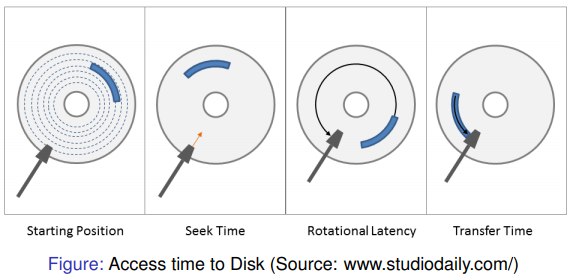
\includegraphics[scale=0.6]{hdd_access.png}
\end{center}
\pagebreak

\begin{flushleft}
\textbf{Multiple requests} may be happening at the same time (\textbf{concurrently}). Thus, access time may be \textbf{increased} by a queueing time. In this scenario, dominance of seek time leaves room for \textbf{optimisation} by carefully considering the \textbf{order} of read operations. The estimated \textit{seek time} (i.e., to move the arm from one track to another) is approximated by: \[T_{s} = n * m  + s \] In which :
\begin{itemize}
	\item $T_{s}$ denotes the \textbf{estimated seek time}
	\item $n$ the \textbf{number of tracks to be crossed}
	\item $m$ the \textbf{crossing time per track}
	\item $s$ any additional \textbf{startup delay}
\end{itemize}
It is important to \textbf{position} the sectors carefully and avoid \textit{disk fragmentation}.
\end{flushleft}

\section{Disk scheduling}
\begin{flushleft}
The OS must use the hardware \textbf{efficiently}: 
\begin{itemize}
	\item The file system can \textbf{position/organise} files strategically
	\item Having multiple disk requests in a queue allows us to \textbf{minimise} the arm movement 
\end{itemize}
Note that every I/O operation goes through a \textbf{system call}, allowing the operating system to \textbf{intercept} the request and resequence it. If the drive (or the controller) is free, the request can be serviced \textbf{immediately}, if not, the request will be \textbf{queued}.\\
In a \textbf{dynamic} situation, several I/O requests will be made over time that are \textbf{kept} in a table of requested sectors per cylinder. Disk scheduling algorithms \textbf{determine} the order in which disk events are processed.
\end{flushleft}

\subsubsection{Algorithms}
\begin{itemize}
	\item First come first served (FCFS)
	\begin{itemize}
		\item perform operations in order requested
		\item no reordering of work queue
		\item no starvation: every request is serviced
		\item poor performance
	\end{itemize}
	\item SSTF (Shortest Seek Time First)
	\begin{itemize}
		\item after a request, go to the closest request in the work queue, regardless of direction
		\item reduces total seek time compared to FCFS
		\item Disadvantages
		\begin{itemize}
			\item starvation is possible; stay in one area of the disk if very busy
			\item switching directions slows things down
		\end{itemize}
	\end{itemize}
	\item SCAN
	\begin{itemize}
		\item keep moving in the same direction until end is reached (start upwards)
		\begin{itemize}
			\item It continues in the current direction, servicing all pending requests as it passes over them
			\item When it gets to the last cylinder, it reverses direction and services all the pending requests (until it reaches the first cylinder)
		\end{itemize}
		\item (Dis-)advantages include:
		\begin{itemize}
			\item The upper limit on the “waiting time” is 2 × number of cylinders, i.e. no starvation occurs
			\item The middle cylinders are favoured if the disk is heavily used (max. wait time is N tracks, 2N for the cylinders on the edge)
		\end{itemize}
	\end{itemize}
	\item LOOK
	\begin{itemize}
		\item like SCAN but stops moving inwards (or outwards) when no more requests in that direction exist.
	\end{itemize}
	\item C-SCAN (circular scan)
	\begin{itemize}
		\item The disk arm moves in one direction servicing requests
		\item When it gets to the last cylinder of the disk, it reverses direction but it does not service requests on the return journey
		\item Once it gets back to the first cylinder it reverses direction, and again services requests
		\item It is \textbf{fairer} and \textbf{equalises} response times across a disk
	\end{itemize}
	\item C-LOOK
	\begin{itemize}
		\item moves inwards servicing requests until there are no more requests in that direction, then it jumps to the outermost outstanding requests.
		\item repeast this over and over.
		\item variant: service requests from inside to outside, then skip back to the innermost request.
	\end{itemize}
\end{itemize}

\section{Driver caching}
\begin{flushleft}
For most current drives, the time required to seek a new cylinder is \textbf{more} than the rotational time (remember pre-paging in this context!). It makes sense, therefore, to \textbf{read more} sectors than actually required. Read sectors during the rotational delay (i.e. that \textbf{accidentally pass by}). Modern controllers read \textbf{multiple sectors} when asked for the data from one sector: \textit{track-at-a-time caching}.
\end{flushleft}

\section{SSD}
\begin{flushleft}
Solid State Drives (SSDs) have no moving parts and store data using electrical circuits. They don’t have \texttt{Tseek} or rotational delay!\\
\textbf{FCFS} algorithm is useful in general purposes systems\\
SSTF, SCAN, LOOK-SCAN may reduce performance (no heads to move)
\end{flushleft}

\section{Notes}
\begin{flushleft}
Take a look at slides for algorithm time calculation examples.
\end{flushleft}

\pagebreak
\section*{Reference section} \label{sec:reference}
\begin{description}
	\item[spindle] \hfill \\ A spindle is a shaft that holds rotating hard disk drive (HDD) platters in place. The term is also often used to refer to a single HDD.
\end{description}
\end{document}
